\begin{frame}{Introduction}
\begin{block}{Definition}
VLMs learn to map the relationships between text data and visual data such as images or videos, allowing these models to generate text from visual input or understand natural language commands in the context of visual information\footnotemark.
\end{block}

\begin{figure}
    \centering
    \includegraphics[width=0.6\linewidth]{images/vision_language_model_outline.png}
    \caption{Visualization of a Vision-Language Model}
\end{figure}

\footnotetext{\url{https://www.ibm.com/think/topics/vision-language-models}}
\end{frame}

\begin{frame}{Introduction}
\begin{block}{Core Capabilities}
\begin{itemize}
    \item Unlike traditional computer vision models, VLMs are not bound by a fixed set of classes or a specific task such as classification or detection.
    \item Retrained on a vast corpus of text and image / video caption pairs, VLMs can be trained in natural language and used to handle many classic vision tasks plus new AI-powered generative tasks such as summarization and visual question answering.
\end{itemize}
\end{block}
\begin{figure}
    \centering
    \includegraphics[width=0.6\linewidth]{images/vision_language_model_outline2.png}
    \caption{Illustrations of Visual Question Answering}
\end{figure}
\end{frame}

\begin{frame}{Introduction}
\begin{figure}
    \centering
    \includegraphics[width=0.6\linewidth]{images/intro_image.png}
    \caption{Three DNN training paradigms in visual recognition.}
\end{figure}
\end{frame}


\begin{frame}{Introduction}
\centering
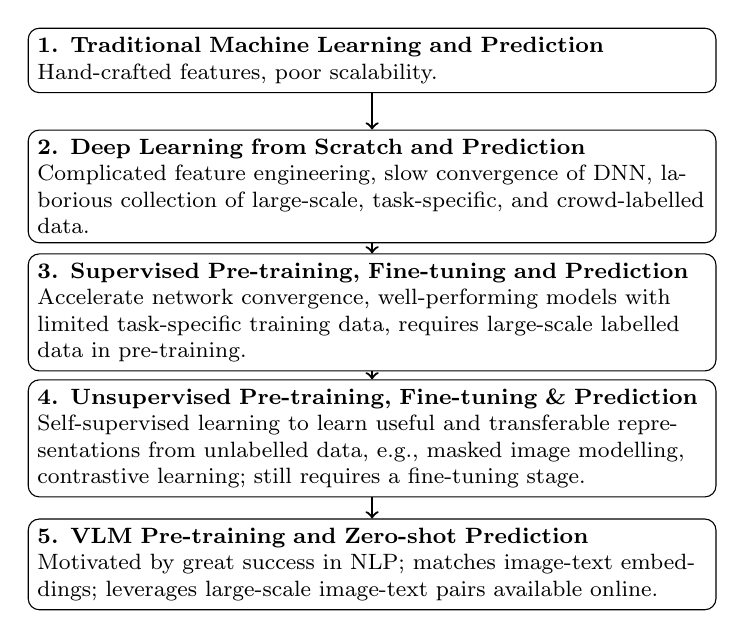
\begin{tikzpicture}[
  node distance=1.6cm,
  every node/.style={rectangle, draw=black, rounded corners, align=left, text width=8.5cm, font=\footnotesize, fill=white},
  line/.style={->, thick, draw=black}
]

\node (block1) {\textbf{1. Traditional Machine Learning and Prediction}\\
Hand-crafted features, poor scalability.};

\node (block2) [below of=block1] {\textbf{2. Deep Learning from Scratch and Prediction}\\
Complicated feature engineering, slow convergence of DNN, laborious collection of large-scale, task-specific, and crowd-labelled data.};

\node (block3) [below of=block2] {\textbf{3. Supervised Pre-training, Fine-tuning and Prediction}\\
Accelerate network convergence, well-performing models with limited task-specific training data, requires large-scale labelled data in pre-training.};

\node (block4) [below of=block3] {\textbf{4. Unsupervised Pre-training, Fine-tuning \& Prediction}\\
Self-supervised learning to learn useful and transferable representations from unlabelled data, e.g., masked image modelling, contrastive learning; still requires a fine-tuning stage.};

\node (block5) [below of=block4] {\textbf{5. VLM Pre-training and Zero-shot Prediction}\\
Motivated by great success in NLP; matches image-text embeddings; leverages large-scale image-text pairs available online.};

% Arrows
\draw [line] (block1) -- (block2);
\draw [line] (block2) -- (block3);
\draw [line] (block3) -- (block4);
\draw [line] (block4) -- (block5);

\end{tikzpicture}
\end{frame}
